\documentclass[journal]{IEEEtran}

% WM-Concord paper draft, Fall 2026, Group 6. Built from the course IEEEtran template.
% Figures come from the report (reports/Latex_report/fig, made by reports/Latex_report/make_figures.py)
% and references from the report's bib file, so both documents always use the same numbers and sources.

\usepackage{amsmath, amsfonts, array, graphicx, booktabs, balance, cite}
\usepackage[colorlinks,linktocpage]{hyperref}
\hypersetup{
   colorlinks   = true,
   urlcolor     = blue,
   linkcolor    = blue,
   citecolor    = red,
   setpagesize  = false,
   linktocpage  = true,
}
\graphicspath{{../../reports/Latex_report/fig/}{Fig/}}

\begin{document}
\raggedbottom

\title{Do World Model Diagnostics Agree?\\ A Cross Diagnostic Validity Study on a Controlled Model Zoo}

\author{Venkatesh~Nagarjuna, Siddardha~Reddy, Nikhil~Obuleni, Viharika~Vemparala, and~Amir~Jafari%
\thanks{The authors are with the Data Science Program, The George Washington University, Washington, DC, USA.}}

\markboth{WM-Concord draft, Fall 2026}{Nagarjuna \MakeLowercase{\textit{et al.}}: Do World Model Diagnostics Agree?}
\maketitle

\begin{abstract}
Claims that sequence models learn a world model of their domain rest on four families of diagnostics: next
token validity, state equivalence, inductive bias probes and representation probing. Each published study uses
one of them, on its own models, and on Othello they reach opposite conclusions. We run all four on the same
controlled zoo of 81 Othello models (three architectures, three scales, three training distributions, three
seeds) under a preregistered analysis, and judge them against a fragility suite frozen before any score. The
diagnostics agree strongly on raw scores (Kendall W 0.87), but almost all of this agreement is shared
competence: with the legal move rate controlled, W falls to 0.27 and no pair of the diagnostics that can be
separated from competence agrees. Their disagreement is not explained by architecture, scale or training data.
Only the representation probe adds to the legal move rate in predicting fragility, and an exploratory analysis
shows that this signal is a difference between training distributions, not a relation among comparable models.
Navigation and a held out program interpreter test whether these findings generalize.
\end{abstract}

\begin{IEEEkeywords}
World models, interpretability, probing, measurement validity, Othello, preregistration.
\end{IEEEkeywords}

\section{Introduction}
\IEEEPARstart{W}{hether} a sequence model trained only to predict the next token builds a coherent internal
model of its domain is a central open question. The same Othello models have been reported both as having a
world model~\cite{li2023othello, nanda2023emergent, yuan2025revisiting} and as lacking a coherent
one~\cite{vafa2024evaluating, vafa2025inductive}. Each of these studies uses its own diagnostic on its own
models, so their disagreement cannot be interpreted. Following the measurement view of Jacobs and
Wallach~\cite{jacobs2021measurement}, we treat ``has a world model'' as a construct and the diagnostics as
competing measures of it, and ask whether they agree (convergent validity) and which predicts failure on shifted
tasks (predictive validity). We propose no new diagnostic.

Our contributions are: the first head to head comparison of four world model diagnostics on the same models and
ground truth; a test of their predictive validity against a fragility suite frozen before any score; and an open
benchmark with a common interface to which future diagnostics can be added.

\section{Related Work}
Representation probing reads the board from activations~\cite{li2023othello}, linearly once squares are labelled
relative to the player~\cite{nanda2023emergent}, and across fine tuned language models~\cite{yuan2025revisiting};
state tracking has been tested behaviourally in chess~\cite{toshniwal2022chess}. Vafa et al.\ derive state
equivalence metrics from the Myhill Nerode theorem~\cite{vafa2024evaluating, nerode1958linear} and propose
inductive bias probes~\cite{vafa2025inductive}. Control tasks~\cite{hewitt2019control} and the limits of
probing~\cite{belinkov2022probing} shape our D4. Benchmarks often claim more than they measure~\cite{raji2021benchmark}.
For inference with repeated runs we follow the cluster bootstrap~\cite{cameron2008bootstrap} and the case for
accounting for seed variance~\cite{bouthillier2021variance}.

\section{Method}
\subsection{Model zoo and domain}
Othello's true state (board and player to move) is replayed exactly by our rules engine. We train
transformers~\cite{vaswani2017attention}, stacked LSTMs~\cite{hochreiter1997lstm} and Mamba~\cite{gu2023mamba}
at three scales (0.48 to 25.3 million parameters) on synthetic, championship (WTHOR) or mixed games, three seeds
each, with one fixed budget. A model is admitted if its validation legal move rate, its \emph{competence}, is
at least 0.50; all 81 are admitted (competence 0.559 to 0.969).

\subsection{Diagnostics}
\textbf{D1} is the share of positions whose top predicted move is legal. \textbf{D2} is one minus the mean of the
compression and distinction errors of Vafa et al.~\cite{vafa2024evaluating} with next move continuations.
\textbf{D3} is the balanced accuracy gain of the pretrained model over a random weight twin when adapted on 64
examples to ``is square $X$ mine?''~\cite{vafa2025inductive}, with a symbolic regression arm~\cite{cranmer2023pysr}.
\textbf{D4} is the selectivity of a linear mine, theirs or empty probe~\cite{hewitt2019control} at the best
layer, with a causal edit check~\cite{li2023othello}. Protocols were tuned only on the two published Othello GPTs.

\subsection{Fragility and analysis}
The fragility suite keeps the rules and shifts the situations (other distributions, after a pass, symmetries,
forced detours); relative fragility divides the mean drop in legal move rate by the model's own rate. All
rules were preregistered with git tags before the results they affect. H1 uses Kendall's tau~\cite{kendall1938tau},
Kendall's partial tau given competence~\cite{kendall1942partial} and Kendall's W~\cite{kendall1939w}; H2 regresses
per model disagreement on the design factors against a seed noise floor; H3 tests D2 to D4 beyond D1 by partial
Spearman correlation. Intervals are 95\% cluster bootstrap intervals over the 27 configurations.

\section{Results on Othello}
\begin{figure}[t]
    \centering
    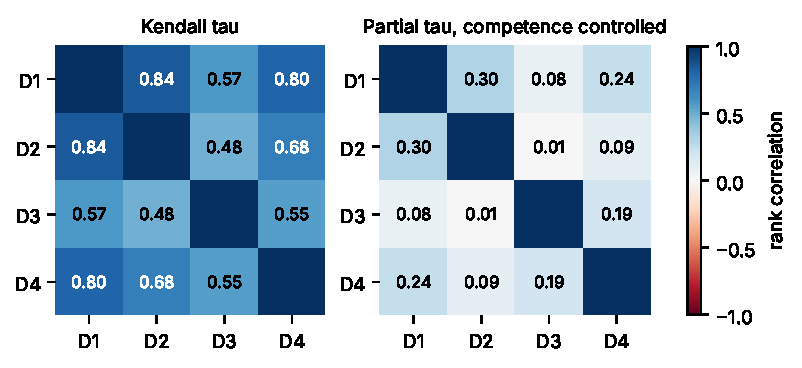
\includegraphics[width=\columnwidth]{othello_h1.pdf}
    \caption{Rank agreement between diagnostics, raw and with competence controlled (81 models).}
    \label{fig:h1}
\end{figure}

\textbf{H1.} Five of six pairs agree on raw scores and W is 0.872 [0.764, 0.921] (Fig.~\ref{fig:h1}). Every
diagnostic follows competence (tau 0.968 for D1, 0.826 D2, 0.790 D4, 0.577 D3). D1 pairs are not interpretable
after the control (preregistered rule), and the three pairs among D2, D3 and D4 all lose their agreement; W on
competence residuals is 0.267 [0.189, 0.427].

\textbf{H2.} Mean disagreement is 0.089 against a seed noise floor of 0.028; no factor is significant after Holm
correction (architecture $p=0.78$, scale $p=0.081$, training data $p=0.34$).

\textbf{H3.} D1 does not predict relative fragility (0.150 [$-0.315$, 0.588]). Only D4 adds to D1 (partial
$-0.554$ [$-0.734$, $-0.124$]), but no single diagnostic wins. In an exploratory analysis, championship trained
models are both the most fragile and the least probe readable (Fig.~\ref{fig:d4}); within each training
distribution the D4 link vanishes, and with training data controlled it is $+0.231$ [$-0.336$, 0.589].

\begin{figure}[t]
    \centering
    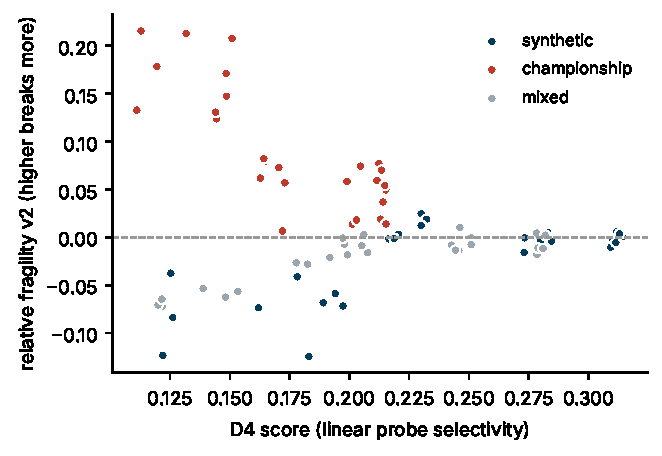
\includegraphics[width=0.9\columnwidth]{othello_h3_d4.pdf}
    \caption{D4 against relative fragility, by training distribution (exploratory).}
    \label{fig:d4}
\end{figure}

\section{Discussion}
On Othello the diagnostics agree mainly because better models score higher on all of them; beyond competence they
measure different things, and none reliably predicts fragility among comparable models. A board that can be read
out is not a board that is used: every model is decodable but only 10 of 81 pass the causal check. Studies that
report a single diagnostic on models of different quality mostly report competence.

\section{Conclusion and Future Work}
We will repeat the analysis on navigation, reproducing the state equivalence results of Vafa et
al.~\cite{vafa2024evaluating}, and test generalization (H4) on a held out program interpreter.

\section*{Acknowledgment}
We thank the GWU Data Science Program for compute on AWS.

\balance
\bibliographystyle{IEEEtran}
\bibliography{../../reports/Latex_report/references}
\end{document}
